\begin{problem}[问题1.3]
若两小固体漂浮在液面上. 试说明, 当两固体均被液体浸润或当它们均不被浸润时, 表面张力
的作用是使相邻两固体相互接近; 当一个是被浸润而另一个不被浸润时, 表面张力是使它们彼此远离.
\end{problem}
\begin{solution}
\begin{figure}[!htb]
\begin{minipage}[b]{.33\textwidth}
\centering
\usetikzlibrary{%
    decorations.pathreplacing,%
    decorations.pathmorphing,arrows
}
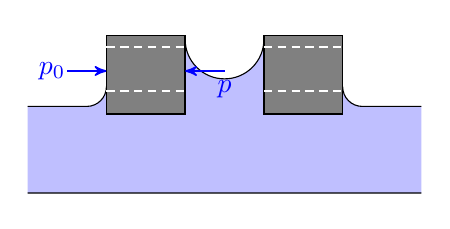
\begin{tikzpicture}
\clip (0,-0.1) rectangle(5,2.1);

\fill[blue!25,draw=black] (-0.1,1.1)--(0.75,1.1) arc(-90:0:0.25)-- (2,1.95) arc(-180:0:0.5)--(4,1.35) arc(-180:-90:0.25)  --(5.1,1.1)--(5.1,0)--(-0.1,0)--cycle;
\draw[semithick,fill=gray] (1,1) rectangle (2,2) (3,1) rectangle(4,2);
\draw[white,densely dashed,thick] (1,1.3)--(2,1.3) (3,1.3)--(4,1.3) (1,1.85)--(2,1.85) (3,1.85)--(4,1.85);
\draw[->,semithick, >=stealth',blue] (0.5,1.55)node[left=-3pt]{$p_0$}--(1,1.55);
\draw[<-,semithick, >=stealth',blue](2,1.55)-- (2.5,1.55) node[below]{$p$};
\end{tikzpicture}
\caption{\label{float01}浸润-浸润}
\end{minipage}%
\begin{minipage}[b]{.33\textwidth}
\centering
\usetikzlibrary{%
    decorations.pathreplacing,%
    decorations.pathmorphing,arrows
}
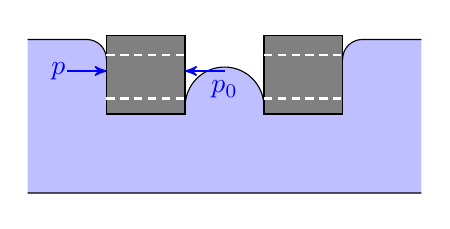
\begin{tikzpicture}
\clip (0,-0.1) rectangle(5,2.1);
\fill[blue!25,draw=black] (-0.1,1.95)--(0.75,1.95) arc(90:0:0.25) -- (2,1.1) arc(180:0:0.5)--(4,1.7) arc(180:90:0.25)  --(5.1,1.95)--(5.1,0)--(-0.1,0)--cycle;
\draw[semithick,fill=gray] (1,1) rectangle (2,2) (3,1) rectangle(4,2);

\draw[white,densely dashed,thick] (1,1.2)--(2,1.2) (3,1.2)--(4,1.2) (1,1.75)--(2,1.75) (3,1.75)--(4,1.75);

\draw[->,semithick, >=stealth',blue] (0.5,1.55)node[left=-3pt]{$p$}--(1,1.55);
\draw[<-,semithick, >=stealth',blue](2,1.55)-- (2.5,1.55) node[below]{$p_0$};
\end{tikzpicture}
\caption{\label{float02}不润湿-不润湿}
\end{minipage}
\begin{minipage}[b]{.33\textwidth}
\centering
\usetikzlibrary{%
    decorations.pathreplacing,%
    decorations.pathmorphing,arrows
}
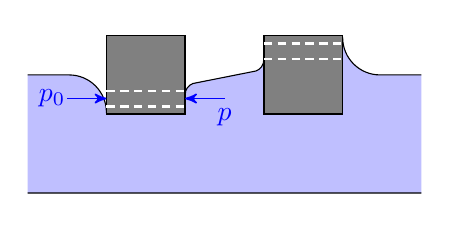
\begin{tikzpicture}
\clip (0,-0.1) rectangle(5,2.1);

\fill[blue!25,draw=black] (-0.1,1.5)--(0.525,1.5) arc(90:0:0.475)-- (2,1.25) arc(180:110:0.15) --(2.9,1.55) arc(-70:0:0.15)--(4,1.975) arc(-180:-90:0.475)  --(5.1,1.5)--(5.1,0)--(-0.1,0)--cycle;

\draw[semithick,fill=gray] (1,1) rectangle (2,2) (3,1) rectangle(4,2);
\draw[white,densely dashed,thick] (1,1.1)--(2,1.1) (3,1.7)--(4,1.7) (1,1.3)--(2,1.3) (3,1.9)--(4,1.9);

\draw[->,semithick, >=stealth',blue] (0.5,1.2)node[left=-3pt]{$p_0$}--(1,1.2);
\draw[<-,semithick, >=stealth',blue](2,1.2)-- (2.5,1.2) node[below]{$p$};
\end{tikzpicture}
\caption{\label{float03}不润湿-浸润}
\end{minipage}
\end{figure}
\textbf{解:}如图\ref{float01}-\ref{float03}所示,是本题中所要考虑的三种情况.当两物块没有接近时,各自在各个方向上受的到表面张力的水平分量相互平衡,竖值分量与重力及浮力平衡, 表现为静止.
当两物块靠近时,
表面张力有缩小两物块间液体的表面积, 至使小物块内外两侧出现压力差
,结果表现为相互接近或远离.下面就这三种情况一一分析:
\begin{enumerate}
\item \textbf{浸润-浸润}:如图\ref{float01}中两物块,当它们靠近时,它
们之间的凹形液面在表面张力的作用下将缩小表
面积使其上升, $p<p_0$, 因此两物块相互接近.
\item \textbf{不润湿-不润湿}:如图\ref{float02}中两物块,当它们靠近时,它
们之间的凸形液面在表面张力的作用下将缩小表
面积使其下降, $p<p_0$, 因此两物块相互接近.
\item \textbf{浸润-不润湿}:如图\ref{float03}中两物块,当它们靠近时,左物块的右侧凸液面及右物块的左侧凹液面在表面张力的作用下缩小表面积,对于左物块有$p>p_0$受得向左的合力, 同样对于右块可知受到向右的合力, 因此它们彼此远离.
\end{enumerate}
\end{solution}
